\documentclass[oneside,12pt]{discsthesisundergrad}
\usepackage{graphicx} % Package for Figures
\usepackage{float} % Package for better control of placing of figures
\usepackage{tabularx} % Package for tables
\usepackage{multirow} % Package for "Merging" of rows in tables
\usepackage[normalem]{ulem} % Package for better control of tables (Wrapping, Column Width)
\usepackage[titletoc]{appendix} % Package for adding Appendices


% Defining new column widths for tables using ulem package. These are just samples.
\useunder{\uline}{\ul}{}
\newcolumntype{L}{>{\raggedright\arraybackslash}m{7.5cm}}
\newcolumntype{M}{>{\raggedright\arraybackslash}m{5.5cm}}
\newcolumntype{S}{>{\raggedright\arraybackslash}m{3.5cm}}
\newcolumntype{R}{>{\raggedright\arraybackslash}m{2.5cm}}

% Declaring the path where Appendices will be placed
\graphicspath{ {Appendices/} }

\begin{document}

 \ThesisAuthor{\textbf{Beatrice Amara E. Adajar \break Jann Railey E. Montalan}}
  \ThesisTitle{\textbf{DEVELOPMENT OF A WEB SCRAPING ALGORITHM ON \\ NEWS SITES FOR SYNDROMIC SURVEILLANCE}}
  \ThesisArea{Computer Science}
  \ThesisDefenseYear{2018}
%  \DefenseDate{14 July 2017}
  %\ThesisGrade{Very Good}
  \ThesisStyle{BS}{draft}{-10pt}{15pt}
  
  \FrontMatter

  
% \begin{thesisabstract}

This is where you will put the abstract. Write something about your paper.

This is a note.

\end{thesisabstract}
\tableofcontents
\listoffigures
\MainMatter

% The \input tag signifies that you would "include" (like in java) the following .tex files.
 \chapter{Introduction}

In compliance with the 2005 revisions of the International Health Regulation (IHR), countries were required to report disease outbreaks of international level to the World Health Organization (WHO) within 24 hours \cite{worldtechnical}. As such, many countries have employed disease surveillance techniques so that outbreak cases could be reported to the respective bodies as soon as possible \cite{hartley2010landscape}.

Many traditional disease surveillance systems have relied chiefly on data generated by various health care workers from private health institutions and the public health system \cite{rohart2016disease}. However, some systems from other countries have been shown to take weeks to properly confirm cases of disease before resolving to an appropriate response \cite{rohart2016disease}, showing a possible problem with timeliness.

Various public health systems have turned towards syndromic surveillance, where signs and symptoms are used to detect disease before confirming diagnoses \cite{mandl2004implementing}, making it a useful tool in the early detection and monitoring of disease outbreaks.

Syndromic surveillance systems use data from electronically available sources such as electronic medical records \cite{lazarus2001using}, but also utilize unstructured sources such as infodemiological (health-related) tweets \cite{espina2016towards}. Moreover, global surveillance systems such as GPHIN, EpiSPIDER, and HealthMap that utilize articles from news sites have also been shown to be effective in generating event-based outbreak information \cite{keller2009use}. Sources such as these provide current and localized information about outbreaks, even from areas that are relatively unnoticed by traditional public health efforts \cite{woodall1997official}.

As such, this study proposes to augment an existing syndromic surveillance effort in the Philippines called FASSSTER through web scraping local news sites for syndromic data. This would allow data readily created by news providers in the Philippines to be used in the early detection of diseases. 

\section{Research Questions}

This study seeks to determine how web scraping local news sites of syndromic data can augment FASSSTER, a syndromic surveillance initiative in the Philippines, in the early detection of diseases.

Specifically, it seeks to answer the following:
\begin{enumerate}
\item What methods of web scraping would allow for retrieving relevant syndromic data from local news websites and utilizing this information for syndromic surveillance?
\item Is the volume of news articles generated by local news sites sufficient enough to be used for syndromic surveillance?
\item How does web scraping syndromic data from local news sites augment FASSSTER in terms of relevance and reliability of data? 
\end{enumerate}
\section{Objectives of the Study}

This study aims to utilize web scraping techniques to retrieve relevant syndromic data from local news sites for use in syndromic surveillance.

More specifically, it aims to do the following:
\begin{enumerate}
\item Identify methods of web scraping local news sites to retrieve syndromic information that can be useful for the early detection of diseases.
\item Demonstrate that the volume of news articles generated by local news sites is sufficient for use in syndromic surveillance. 
\item Identify the value of web scraping local news sites in terms of retrieving relevant and reliable syndromic data.
\end{enumerate}
\section{Scope and Limitations}

This study focuses on syndromic surveillance, which uses syndromic data that is composed of identified signs and symptoms that are not necessarily confirmed through appropriate means of diagnoses by doctors. It will not focus on other means of epidemic intelligence such as indicator-based surveillance. 

This study will only focus on syndromic data that can be mined from health-related news articles published by local news sites. It will not tackle other sources of data such as infodemiological social media posts, electronic medical records, or other health-related media. 

Furthermore, this study will only focus on FASSSTER, a syndromic surveillance system developed by the Ateneo Java Wireless Competency Center. It will not seek to create a separate surveillance system altogether.
\section{Significance of the Study}

The study utilizes computer science concepts such as web scraping, support vector machines, latent Dirichlet allocation, relational databases, and system integration. Local news sites will be web scraped to retrieve news articles. These articles will then be subjected to support vector clustering to separate those that contain syndromic data from those that do not, then be further subjected to topic modeling through latent Dirichlet allocation. Information from this will then be stored in a relational database, and shall then be integrated into FASSSTER, an existing syndromic surveillance system.

This study could contribute to the improvement of syndromic surveillance systems employed in the Philippines. News sites generate relevant and crucial data that relate to health events, and this study aims to make use of this data for the earlier detection of diseases. This proposed system has the potential to give way to better syndromic surveillance efforts in the country. 
 \chapter{Review of Related Literature}

% Add a brief overview of each section/subsection of your RRL. 

This research concerns itself with two major components, namely concepts related to web scraping and its relation to syndromic surveillance. 

\section{Disease Surveillance in the Philippines}

%BEAAAAAAA
%I think you can use the Epidemic Intelligence framework literature from our last paper

Disease surveillance is key to the identification and monitoring of potential health risks used for determining appropriate responses to be undertaken for public health control measures \cite{doh2014manual}.

The Department of Health (DOH) employs the Philippine Integrated Disease Surveillance and Response (PIDSR) system which is “a process of coordinating, prioritizing, and streamlining of multiple disease surveillance systems into a unified national disease surveillance system” \cite{doh2014manual}. According to the PIDSR manual, its integrated disease surveillance efforts work on a framework that emphasizes 6 core activities: detection, registration, reporting, confirmation, analysis and feedback. The system uses various systems including case-based, laboratory-based, event-based, and indicator based surveillance approaches, done in concurrence local government units and partner private health institutions \cite{doh2014manual}.

In tangent with this, the Philippines adopted the National Objectives for Health 2005-2010 and 2011-2016, that ``prioritized ICT in various reforms areas, critical health programs, and specific areas in health administration'' \cite{doh2014ehealth}. In 2014, DOH also introduced the Philippine eHealth Strategic Framework and Plan 2020 in 2014 \cite{doh2014ehealth}, establishing guidelines in implementing electronic public health systems. There are several components needed in ``achieving a national eHealth environment in the country'' shown in Figure \ref{fig:eHealth} \cite{doh2014ehealth}. For this study, it will focus on eHealth Solutions, in particular, \textit{Information Sources}. 

\begin{figure}[H]
    \centering
    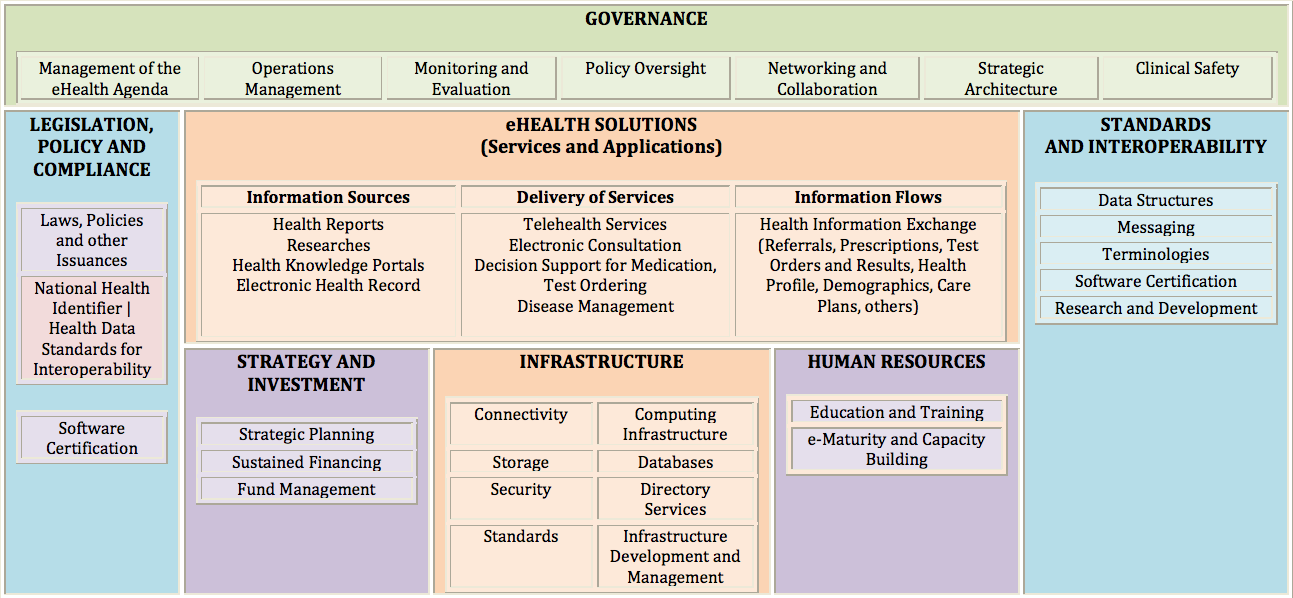
\includegraphics[width=\textwidth]{eHealth}
	\caption{eHealth Component Map from the Philippine eHealth Strategic Framework and Plan 2020 \cite{doh2014ehealth}.}
	\label{fig:eHealth}
\end{figure}
\section{Syndromic and Spatial Surveillance}
Surveillance systems use various methods to monitor public health. One approach is to identify syndromes--groups of health signs and symptoms that coexist frequently together \cite{doh2014manual}--given a duration and population to identify the existence of diseases. This approach, called syndromic surveillance, detects possible outbreaks through identifying trends that demonstrate such signs and symptoms that occur in a given area and time. Syndromic data is acquired from various non-automated (medical logs, emails, and others) and automated means (data files, databases, and others) and are transmitted and stored, and integrated with other syndromic data for analysis and response \cite{mandl2004implementing}.

Another approach is to identify the extent of ``clusters'' of similarly attributed cases across a map. This cluster detection is central to spatial surveillance, and involves the plotting of health information that specifies its location through geocodes such as zip or postal codes, or geographical information such as exact latitudes and longitudes \cite{lawson2005spatial}. Lawson states that as outbreaks are ``localized at some spatial scale,'' spatial surveillance will be able to detect spikes in health events over a small area \cite{lawson2005spatial}.

As such, syndromic and spatial surveillance techniques are used to identify what Lawson describes as ``changes in public health [that] might trigger interventions'' \cite{lawson2005spatial}. Methods have been developed to detect these changes, such as statistical process control (SPC) \cite{oakland2007statistical} and cumulative sum (CUSUM) \cite{fricker2008comparing}. These deal with factors such as changepoints (statistical nonparametric values), clusters, and overall process change. 


%aggregated score for a health index that is a "symptom" for a particular disease

\subsection{FASSSTER}
Feasibility Analysis of Syndromic Surveillance Using Spatio-Temporal Epidemiological Modeler for Early Detection of Diseases (FASSSTER) is a system created by the Ateneo Java Wireless Competency Center in partnership with the Department of Health and the Department of Science and Technology — Philippine Council for Health Research and Development. It integrates various data sources on health and the spread of diseases to create appropriate models and visualizations \cite{fassster}.

Currently, for syndromic surveillance, FASSSTER integrates data from the following sources: SHINE OS+, infodemiological (or health-related) tweets, and Philippines Integrated Disease Surveillance and Response (PIDSR) \cite{fassster}. 

Infodemiological tweets are gathered through a tool that utilizes the Twitter API, and the tool captures tweets based on specific health-related keywords. The tweets are then filtered to only include those in the Filipino language and those that are not retweets, then classified if whether or not they are relevant to infodemiology \cite{espina2016towards}.

FASSSTER uses IBM's Spatio-Temporal Epidemiological Modeler (STEM), a tool used to simulate the spread of disease. STEM contains the following components \cite{edlund2010spatiotemporal}:
\begin{enumerate}
\item \textit{Graphical user interface} to allow users to interact with the tool; 
\item \textit{Representational framework} that uses graphs to describe locations of populations and the risk of spreading; and 
\item \textit{Disease model computations} that model infectious diseases described by several differential equations \cite{anderson1992infectious}.
\end{enumerate}
\section{Web-based Disease Surveillance}

Early and timely detection of disease outbreaks ushered the rise of newer technologies that could augment existing systems of disease surveillance \cite{chunara2012new}. Web-based technologies in particular have been shown to provide ``greater communication and improved surveillance and reporting frameworks,'' improving the timeliness of outbreak detection \cite{chan2010global}. Such surveillance systems are also ``intuitive, adaptable, low-cost, and [operate] in real-time'' \cite{choi2016web}, ``with reduced cost and increased reporting transparency'' \cite{wilson2009early}. This demonstrates the advantages of using such approaches in disease detection. 

A study by Choi \textit{et al.} lists down several web-based technologies that have been employed for identifying emerging infectious diseases, shown in Figure \ref{fig:webbased} \cite{choi2016web}. Most of these systems utilize text mining social media posts and news reports online \cite{brownstein2009digital}. 

\begin{figure}[t]
    \centering
    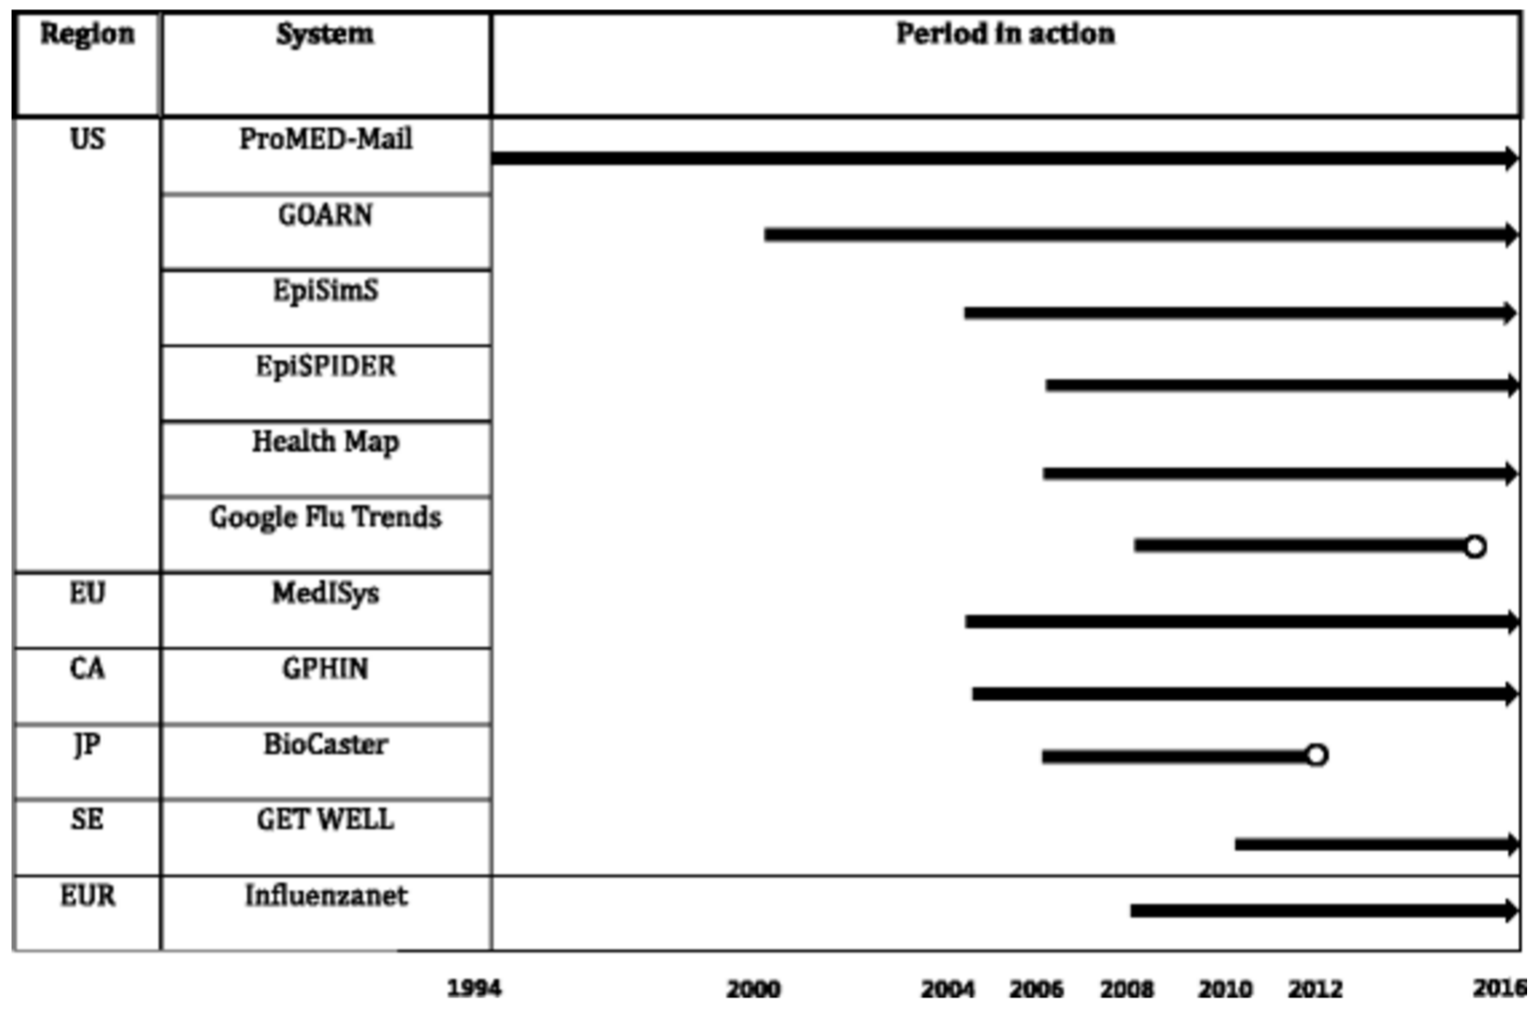
\includegraphics[width=\textwidth]{WebBasedSurveillance}
	\caption{Development of web-based surveillance systems in chronological order \cite{choi2016web}.}
	\label{fig:webbased}
\end{figure}

It has been shown that tweets can be useful in retrieving health-related information generated by users. One study demonstrated an algorithm that can capture tweets and classify them to ascertain if they are ``infodemiological'' (and can be epidemiological purposes) or otherwise \cite{espina2016towards}. Another study presented a topic model for Twitter ``that associates symptoms, treatments and general words with diseases'' \cite{paul2012model}. Both concluded that it is feasible to extract health information from tweets. Multiple studies have also implemented mining health information from tweets, concluding that crowd-source social media-based monitoring tools can provide ``timely information about the state of an epidemic'' \cite{lampos2010tracking, boulos2011crowdsourcing}.

User-generated health information could lead to more expedient recognition of public health events \cite{velasco2014social} through this rapid generation of information, faster than collection of health information from individual health workers in traditional surveillance systems.

Other sources of unstructured information such as Internet news sites have been shown to be relevant in providing ``detailed local and near-real time data on disease outbreaks'' \cite{heymann2001hot,madoff2005internet,morse2007global}. As such, news sites have been used by event-based global surveillance systems such as Global Public Health Intelligence Network (GPHIN), HealthMap, and EpiSPIDER \cite{keller2009use}. The aforementioned systems acquire news articles through Really Simple Syndication (RSS) feeds, news aggregators and news wires, electronic mailing lists, and web scraping techniques. These systems then subject gathered articles to clustering, linguistic analysis, and cross-referencing with other sources to determine their accuracy and relevance \cite{keller2009use}. 

Moderated reporting and information dissemination systems such as the Program for Monitoring Emerging Diseases (ProMED-Mail) and Global Outbreak Alert Response Network (GOARN) also integrate news sites to facilitate networked discussion towards an ``international coordinated response to outbreaks'' \cite{choi2016web}.

\section{Retrieving information from websites}

The web is littered with unindexed and freeform text that are usually not machine-readable, causing these to be ``inaccessible to automated knowledge discovery techniques'' \cite{soderland1997learning}. Despite this, crucial information can still be extracted from websites. Within these unstructured texts are systematic information such as names, dates, and figures that are desirable for a variety of purposes \cite{munzert2014automated}.

\subsection{Web Scraping}
A process that can retrieve such information is called web scraping, and involves fetching web pages then extracting data from them through ``parsing [web pages] and extracting out data points relative to their structure'' \cite{penman2009web}. Web scraping converts this unstructured data (usually in the form of HTML or XML pages), into information that is stored in databases for analysis \cite{vargiu2012exploiting}. Web scraping involves the following processes \cite{munzert2014automated}:

\begin{enumerate}
\item Gathering unstructured data; 
\item Determining noticeable patterns behind the desired information;  and
\item Apply such patterns to unstructured data to extract information
\end{enumerate}

One technique that can be used to scrape data from websites uses automatically generated wrappers for parse HTML files to extract the desired information \cite{crescenzi2001roadrunner}. The technique follows \textit{ACME}:
\begin{enumerate}
\item \textit{Align} HTML code from two HTML pages;
\item Iteratively \textit{Collapse} under \textit{Mismatch}, to find mismatches specified by the wrapper to find common regular expressions between the two pages; and
\item \textit{Extract} data by parsing the text that remains.
\end{enumerate}

\subsection{Data Classification and Topic Modeling}
Before this extracted data can be useful, it should be refined further into data relevant to the purposes through classification and topic modeling techniques.

The problem of data classification, according to Aggarwal, can be stated as follows: ``Given a set of training data points along with associated training labels, determine the class label for an unlabeled test instance'' \cite{aggarwal2014data}. With such a problem, there are normally two phases. The first one, the training phase, deals with constructing a model from a given training dataset. The second one, the testing phase, deals with using the constructed model to assign labels to unlabeled test data points. The end result should be that all unlabeled test instances are correctly labeled by the classifier \cite{aggarwal2014data}.

Probabilistic topic modeling is a set of algorithms designed to allocate documents of text to specific themes or topics. They analyze the text, draw connections between words and themes, and use that to group documents under the generated themes. These algorithms can be adapted to different kinds of data, whether structured or unstructured \cite{blei2012probabilistic}.

With that, data classification and topic modeling techniques could be used to determine correlations between symptoms with ailments \cite{paul2012model} found in web scraped articles that could be potentially useful in syndromic surveillance. 
















 \chapter{Methodology}

\section{Web Scraping News Sites}
The articles will come from mainstream news sites such as GMA News, ABS-CBN News, The Philippine Daily Inquirer, The Philippine Star, Manila Bulletin, and Rappler. These news sites were chosen from the list top Philippine sites generated by Amazon's Alexa. Alexa calculates the top sites globally, by country, or by category, based on daily time on site, daily page views per visitor, percentage of traffic from search, and the total number of sites linking in \cite{alexa}.

Web scraping can be done using a Python framework known as Scrapy. Scrapy is an open-source framework used for extracting data from various web sources. It has multiple components such as a spider engine, which handles the data flow and triggers actions depending on events, spiders, which handle the extraction and parsing of data, and the item pipeline, which then processes the data from the spiders \cite{nisafani2017eliciting}.

Scrapy will be used to pull the articles from the web pages of the given local news sites. These articles will then be classified appropriately using Support Vector Machines and Latent Dirichlet Allocation.
\section{Support Vector Machines}
Support Vector Machines (SVMs) are hyperplanes that divide a given dataset into two sections. All vectors to the left of the hyperplane are denoted as -1, while those on the right are 1. The vectors that lie closest to the hyperplane are known as the support vectors. Moreover, the hyperplane divides the training set in such a way that the margin between the hyperplane and the training vectors is maximized \cite{tong2001support}.

One notable feature of SVMs is the kernel. The kernel function is used to project the given dataset into a higher dimension when necessary, making it possible to find a hyperplane to divide linearly-inseparable data sets \cite{tong2001support}, making the problem a quadratic optimization problem with one global solution. This gives the algorithm a computational advantage not present in some other classification methods \cite{ben2001support}.

SVMs will be used to classify the articles into health-related and non-health-related. Only the health-related articles will be included in the final database of information.

\section{Latent Dirchlet Allocation}
Latent Dirichlet Allocation (LDA) is a probabilistic framework for modeling and classifying collections of discrete data. Topics are represented as a multinomial variable, with each word in a given document allocated to a specific topic. To classify new documents, the probability of each document belonging to a specific topic is calculated using the model generate during the allocation of words to topics \cite{blei2002latent}.

LDA will be used for modeling topics under health and subsequently classifying the health-related articles into specific topics. The resulting percentages from the LDA will also determine the relevance of the article (i.e., if the article in question is really about health or barely) and reliability (i.e., what percentage of the article actually falls under the topic it was classified under). These classified articles will be sent to the database for integration to FASSSTER.
\section{Integration into FASSSTER}
Because FASSSTER's objective is to create a data hub from various health-related sources, web scraping is a viable option as an additional source.

The Spatio-temporal Epidemiological Modeler (STEM) within FASSSTER uses a compartmental disease model that incorporates several sources of syndromic information as coefficients in the differential equations used to model the spread of disease.

Information extracted as a result of web scraping will be stored in a relational database, MongoDB. Afterwards, this information will be directly incorporated as a coeffecient in the differential equation modeler of FASSSTER. 

% We use the plain bibliography style for thesis
\bibliographystyle{plain}

% This is your bib file. Just compile every reference you have to this file. You can copy and paste Bibtex references from Google Scholar, and LaTeX will take care of the formatting. :)
\bibliography{Bibliography}


\end{document}